\chapter{Mobile Agents}
\minitoc

\phantom{c}\side{Mobile agents} are agents that are capable of transmitting themselves, their program and their state, across a computer network, and recommencing execution at a remote site.

The program in this way can choose when and where to migrate, therefore suspending its execution at an arbitrary point and transport itself to another machine where it would resume execution.

The original motivation behind mobile agents is fairly simple: the idea was that mobile agents would replace remote procedure call as a way for processes to communicate over a network.\\



\section{Remote Procedure Calls vs Mobile Agents}
\subsection{Remote Procedure Calls}

With remote procedure calls the idea is that one process can invoke a procedure (method) on another process which is remotely located.

Suppose one process $A$ invokes a method $m$ on process $B$ with arguments $args$; the value returned by process $B$ is to be assigned to a variable $v$. This mechanism can be summarized with the notation:
\[v = B.m(args)\]
Crucially, in remote procedure calls, communication is \side{synchronous}, i.e. process $A$ blocks from the time it starts executing the instruction until the time that $B$ returns a value. If $B$ never returns a value, because the network fails, then $A$ may remain indefinitely suspended, waiting for a reply that will never come.\\
The network connection between $A$ and $B$ may well also remain open, and even though it is largely unused (no data is being sent for most of the time), this may be costly.

In other terms, remote procedure calls enable one computer to call procedures in another. In order to do so however, the two computers must agree in advance upon a protocol: the effects of each remotely accessible procedure and the types of its arguments and results.

Each interaction entails two acts of communication: request and acknowledge, which, consequently, means that the ongoing interaction requires ongoing remote communication.

The overall general architecture is depicted in the following figure:

\begin{figure}[!h]
\centering
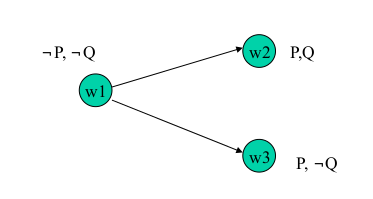
\includegraphics[width=.5\textwidth]{09/00}
\end{figure}

\subsection{Remote execution}
The idea of mobile agents is to replace the remote procedure call by sending out an agent to do the computation. Thus instead of invoking a method:
\begin{enumerate}
\item Process $A$ sends out a program/a mobile agent to process $B$.
\item the program then interacts with process $B$
\item Since the agent shares the same address space as $B$, these interactions cas be carried out much more efficiently than if the same interactions were carried out over a network.
\item When the agent has completed its interactions, it returns to $A$ with the required result.
\end{enumerate}

During the entire operation, the only network time required is that to send the agent to $B$, and that required to return the agent to $A$ when it has completed its task.

This is potentially a much more efficient use of netwrok resources than the remote procedure call alternative.

One computer not only calls procedures on another computer, but also provides the procedures. Hence each exchanged message contains the procedure and its arguments.

The two computers agree in advance upon a language, i.e. instructions and the types of data that are allowed.\\
A user agent and a server can interact without using the network once the agent is transported which means that the ongoing interaction does not require ongoing remote communication.

In the frame of reference of remote executing a mobile agent is a program that can migrate from machine to machine in a heterogeneous network. Moreover, the program is able to choose when and where to migrate and in doing so it will suspend its execution at an arbitrary point, transport itself to another machien and resume execution.

The distintion at the core between pure mobile agents and remote execution is that:
\begin{enumerate}
\item A program which is sent without execution state to remote CPU executes there, possibly communicating with other CPUs and then terminates (remote execution)
\item A program which carries execution state with it and is sent to a remote CPU executes there possibly communicating with other CPUs and then moves again to a third CPI or return to its origin (mobile agent)
\end{enumerate}

\subsection{Advantages of RE over RPC}
We can distinguish to main classes of advantages of remote execution over remote procedure calls:
\begin{enumerate}
\item \side{Tactical}:
\begin{itemize}
\item \side{Performance}: due to less message passing over the network
\item \side{Less connection time}: need network conneciton only to transport the agent
\end{itemize}
\item \side{Strategic}:
\begin{itemize}
\item \side{Customization}: agents let manufacturers of client sw extend the funcitonslities of the server sw.
\item In a RPC application, the server component needs to be statically installed by the user. In RE, they are dynamically installed by the application itself which is an agent.
\item The use of new RPC-based applications must be a decision that has to be taken by the providers.\\
The use of new RE-based applications must be a decision that has to be taken by the user.
\item A public network becomes like a platform
\end{itemize}
\end{enumerate}

\section{Mobile Agent Environment}
A mobile agent environment is a software system which is distributed over a network of heterogeneous computers. Its primary task is to provide an environment in which mobile agents can execute.\\
It implements the majority of models which appear in the mobile agent definition.

A mobile agent environment is responsible to:
\begin{itemize}
\item Support services related to the mobile agent environment itself
\item Support services pertaining to the environments on which the mobile agent environment is built
\item Provide services to support access to other mobile agent systems
\item Provide supp9ort for openness when accessing non-agent-based software environments
\end{itemize}

\section{Issues with Mobile agents}
There are a number of technical issues that arise when considering mobile agents:
\begin{itemize}
\item \side{Serialization}, how is the agent serialized (i.e. encoded in a form suitable to be sent across the network), and, in particular, what aspects of the agent are serialized, the program, the data, or the program and its data?
\item \side{Hosting and remote execution},what the agent arrives at its destincation, how is it executed, for example ifg the original host of the agent employs a different operating system or processor from the desitination host?
\item \side{Security}, when the agent freom A is sent to the computer that hosts process B, there is obvious potential from the agent to cause trouble. It could potentially do this in a number of ways:
\begin{itemize}
\item It might obtain sensitive information by reading filestore or RAM directly
\item It might deny service to other processes on the host machine, by either occupying too much of the available processing resource (processor cycles or memory) or else by causing the host machine to malfunction (e.g. writing over the machine's RAM)
\item It might simply cause irritation and annoyance , for example by causing windows to pop up on the user's GUI
\end{itemize}
\end{itemize}
Many different answers have been developed to address these issues.


With respect to the first issue, that of how to serialize and transmit an agent there are several possibilities:
\begin{itemize}
\item Both the agent and its state are transmitted and the state includes the program counter.

In this way, the agent ``remembers'' where it was before it was transmitted across the network, and when it reaches its destination, it recommences execution at the program instruction following that which caused it to be transmitted
\item The agent contains both a program and the values of variables, but not the program counter, so the agent can remember the values of all variables, but not where it was when it trransmitted itself across the network.
\item The agent to be transmitted is essentially a script, without any associated state (although state might be downloaded from  the original host once the agent has arrived at its destination).
\end{itemize}

\subsection{Security}
The issue of security dominates discussions about mobile agents, in fact we can say that security is a significant concern with mobile agent-based computing.\\
The key difficulty is that, in order for an agent to be able to do anything useful when it arrives at a remote location, it must access and make use of the resources supplied by the remote host. However, provinding access to these resources is inherently dangerous: it lays open the possibility that the host will be abused in some way.

Some general issues in using agents are:
\begin{itemize}
\item \side{Delegation}: you are delegating to the agent some of your authority. This means that agents are doing things that you cannot always see.
\item \side{Mobility}: they may be doing it on the other side of the planet. Or, an agent from the other side of the planet may be doing it on your server
\item \side{Viruses}: mobile agents share many characteristics with viruses. In creating an environment for agents, there is the additional risk that we expose weaknesses that may enable viruses to breed
\item \side{Trust}: humans have classified their co-workers into those who are reliable and those who are not.
\end{itemize}

\subsubsection{Delegation}
The purpose of an agent is to perform some tasks that would otherwise be performed by its user.\\
The agent may need many, if not all, of the access rights of the user.\\
In a security environment, this can be readiliy achieved by passing the copy of the user's certificate to the agent.\\
In this regard, the agent is indistinguishable from any other applications employed by the user.\\
The certificates arte valid for a finite period, defined by the security administrators.

Performing the full delegation is not a big problem. However, a problem is to limit delegated authority.\\
An agent is more flexible and unpredictable than a traditional application.
\subsubsection{Viruses}
It is impossible, in principle, to verify with complete cenrtainty if an arbitrary program is a virus or not.\\
In practice, the problem of writing a program that can verify the correct behaviour of another program is unsolved.\\
It is difficult to define the necessary and sufficient tests that an agent must pass in order to determine its intentions.\\
Some prevautions that can be enforced are: 
\begin{itemize}
\item restriction of access to critical resources
\item restriction on altering other programs
\end{itemize}
\subsubsection{Security for hosts}
In order to enforce security of hosts, the designer needs to design a system that:
\begin{itemize}
\item \side{Limits delegation}.\\
In other terms give the agent and the user separate identities.\\
A way to enforce this limitation is via Secure co-processors: have a physically separate processor on which the agent runs execute the agent in a padded cell.\\
As a result, the approach allows the agent to interact with the system environment only in a language with limited system level expressiveness
\item \side{Limits resource consumption}.\\
In particular, enforcing a limit on the amount of each resource that an agent is permitted to consume or a limit on the amount of budget/CPU time an agent can access.
\end{itemize}
\subsubsection{Security for Agents}
On the contrary we need to protect mobile agents form malicious hosts because:
\begin{itemize}
\item agents have a right to privacy
\item We often do not want to send our programs to a remote host, as to do so might enable the recipient to determine, its purpose and hence our intent
\item the agent might be modified (sabotaged) in some way, without the owner's knowledge or approval
\end{itemize}

In practive, however, the current consensus is that it is computationally impossible to protect a mobile agent form malicious host.

In fact:
\begin{itemize}
\item the use of authentication of the executing server is easy to implement for a single host but quickly becomes difficult for multiple dynamic hosts
\item enforcing agent privacy would require its execution in a highly trusted environment, which consequently would require encapsulating all methods and data and high protection in a Multi agent environment
\end{itemize}

Still there are some possibilities for protection:
\begin{itemize}
\item \side{Data integrity}\\
an agent can be protected in transit by using conventional encryption techniques
\item\side{Origin authentication}\\
certification
\item \side{Access itinerary control}\\
restriction on visiting some environments
\item \side{Privacy and integrity of gathered information}\\
via stateless gathering or stateful gathering
\end{itemize}
\section{Requirements for Mobile Agents}

From the previous sections we can conclude that the general requirements to mobile agent environments are:
\begin{itemize}
\item Expressiveness as a programming language
\item ability to execute remotely or to transport state
\item Support for agent communication language
\item Security support
\item Management support
\end{itemize}